\chapter{\LaTeX \, KULLANACAKLAR İÇİN ÖNERİLER}\label{latexchapter}
\thispagestyle{empty} % pour effacer le numero de page

\section{\LaTeX \, EDİTÖR}
Eğer \LaTeX \, kullanmaya alışkın değilseniz, overleaf gibi online editörler kullanmanız tavsiye edilir, bu şekilde kullanacağınız paketleri teker teker kendiniz indirmek veya eklemek zorunda kalmazsınız. Ayrıca danışmanlarınıza doğrudan link göndererek onların da aktif bir şekilde dosya üzerinde düzeltme yapmalarını sağlayabilirsiniz. 

\section{\LaTeX \, KOMUTLARI}

\subsection{Bölümler ve Bölüm Başlıkları}
Bitirme projesini oluşturan bölümleri \texttt{.tex} uzantılı ayrı dosyalara kaydedip modüler bir şekilde çalışabilirsiniz. 

Projenizi oluşturan her bir bölüm $\backslash$\texttt{chapter} komutuyla oluşturulur, ikinci seviye başlıklar $\backslash$\texttt{section}, üçüncü seviye $\backslash$\texttt{subsection} ve dördüncü seviye başlıklar $\backslash$\texttt{subsubsection} komutları kullanılarak oluşturulur.

Ayrıca bu komutların sonuna $\backslash$\texttt{label\{etiket\}} komutunu ekleyerek, raporunuzun herhangi bir aşamasında daha önceki ya da daha sonraki başlıklara $\backslash$\texttt{ref\{etiket\}} komutu ile metin içerisinden gönderme yapabilirsiniz. Mesela: 
Latex kullanımı ile ilgili öneriler için bkz. Bölüm \ref{latexchapter}.

\subsection{Şekiller}
Kullanılan şekiller, dosyaya ``\texttt{figure}'' ortamı kullanılarak eklenir. Bu şekilde eklenen tüm resimler ve resim yazıları otomatik olarak Liste des Figures başlığı altında görüntülenir. Eklenen resim dosyasına metin içerisinden gönderme yine $\backslash$\texttt{ref\{etiket\}} komutu ile yapılır. Mesela:
\figurename~\ref{fig:lena}'de yer alan resim, görüntü işleme alanında standart test imgesi olarak yaygın kullanıma sahiptir.

\begin{figure}[t]
\centering
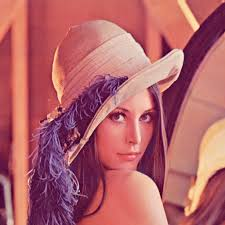
\includegraphics[width=.65\linewidth]{figures/lena.jpg} % Vous devez écrire les extensions des fichiers si vous avez des fichiers de différent types (jpg, png, etc...)
\caption{La photo de Lena Söderberg}\label{fig:lena}
\end{figure}

\figurename~\ref{fig:subfig}'de tek bir Figure etiketi altında birden fazla resim yer almaktadır ve her birine ayrı bir şekilde referans verilebilir (bkz.\figurename~\ref{fig:1a},~\ref{fig:1b},~\ref{fig:1c}). 

\begin{figure}[!h]
\begin{subfigure}[b]{.35\linewidth}
\centering 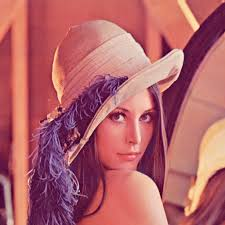
\includegraphics[width=.5\linewidth]{figures/lena.jpg}
\caption{Lena}\label{fig:1a}
\end{subfigure}%
\begin{subfigure}[b]{.35\linewidth}
\centering 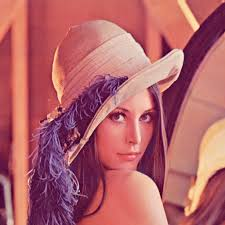
\includegraphics[width=.5\linewidth]{figures/lena.jpg}
\caption{Encore Lena}\label{fig:1b}
\end{subfigure}%
\begin{subfigure}[b]{.35\linewidth}
\centering 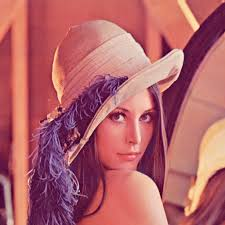
\includegraphics[width=.5\linewidth]{figures/lena.jpg}
\caption{Toujours Lena}\label{fig:1c}
\end{subfigure}
\caption{Une figure avec 3 Lena comme subfigures}\label{fig:subfig}
\end{figure}

\subsection{Tablolar}
Kullanılan tablolar, dosyaya ``\texttt{table}'' ortamı kullanılarak eklenir. Bu şekilde eklenen tüm tablolar ve üst yazıları otomatik olarak Liste des Tableaux başlığı altında görüntülenir. Eklenen resim dosyasına metin içerisinden gönderme yine $\backslash$\texttt{ref\{etiket\}} komutu ile yapılır. Mesela:
\tablename~\ref{tab:tableau}'de örnek bir tablo görüntülenmektedir. 

\begin{table}
\caption {Un tableau} \label{tab:tableau}
\centering
\begin{tabular}{|c|c|c|}
\hline
\textbf{1ere colonne} & \textbf{2eme colonne} & \textbf{3eme colonne} \\\hline
(1,1) & (1,2) & (1,3)\\\hline
(2,1) & (2,2) & (2,3)\\\hline
(3,1) & (3,2) & (3,3)\\\hline
\end{tabular}
\end{table}

Farklı yapılardaki tablo örnekleri Annexes'te mevcuttur, buradaki örnekler \cite{latextables} isimli websitesinden alınmıştır.

\subsection{Denklemler}
Denklemler için ``\texttt{equation}'' ortamı kullanılır. Denklem bir satırı aşıyorsa ``align'' ortamının kullanılması hizalama açısından daha faydalı olacaktır. Örnek: 
\begin{equation}\label{eq:birsatir}
f(x) = ax^3 + bx^2 + cx +d
\end{equation}
\begin{align}\label{eq:coksatir}
P+Q &= 3x^2-2x+5xy-2-3x^2+3x+4x^2+8 \\
P+Q &= x+5xy+4y^2+6
\end{align}

Satır içinde kullanacağınız matematiksel ifadeleri iki \$ işareti arasında yazıp görüntüleyebilirsiniz. Ör: $f(x) = ax^3 + bx^2 + cx +d$

\subsection{Kaynakça}
Kaynakça 2 farklı şekilde oluşturulabilir:
\subsubsection{Elle Kaynakça Oluşturmak}
Latex'de elle kaynakça oluşturmak da mümkündür ama üniversitenin istediği referans formatına uymadığı için, şu an dosyaya da kullanılan \texttt{.bib} uzantılı bibliyografi dosyasını kullanmanız tavsiye edilir.

\subsubsection{Bib Uzantılı Dosya ile Kaynakça Oluşturmak}
Projeniz için kullanacağınız kaynakların \texttt{.bibtex} formatlı dosyalarını internetten hazır bir şekilde bulup, \texttt{.bib} uzantılı dosyanıza ekleyebilirsiniz. Görsel olarak kolaylık sağlayan ve zorunlu ya da gerekli alanların doldurulması konusunda yardım eden Jabref, Zotero, vs.. gibi çeşitli programlar da kullanabilirsiniz. 

Aşağıda \texttt{natbib} paketi ve \texttt{apalike2} isimli referans formatı kullanılarak verilmiş bir kaç alıntı mevcuttur (bu örnekler referans verilen çalışmaların içeriklerinden bağımsız bir şekilde benim tarafımdan uydurulmuştur):

Eğer yazar adını kullanarak referans vermek istiyorsanız, $\backslash$\texttt{citet\{etiket\}} komutunu kullanabilirsiniz. Ör: \citet{konf-bildirisi1} ve \citet{makale2} çalışmalarında ... 

Cümle içinde yazar adını geçirmeyecekseniz, $\backslash$\texttt{citep\{etiket\}} komutunu kullanabiirsiniz.  Ör: ... konu alan başka bir çalışmada elde edilen sonuçlar ... göstermektedir~\citep{makale1}.

Ayrıca aynı komut içerisinde birden fazla referans vermek de mümkündür, bunun için $\backslash$\texttt{citep\{etiket1,etiket2,...etiketn\}} komutunu kullanabilirsiniz. Ör: ... yapılan çalışmalar ... göstermektedir~\citep{kitap1,kitapbolumu1,kitap2,tez1}.

Web sitesi ya da elektronik kitap gibi online olarak yayınlanan kaynaklara atıfta bulunmak için ise oluşturacağınız \texttt{.bib} dosyasını ona göre düzenlemeniz gerekir. Bu kaynakların üniversitenin istediği kaynakça formatına uygun hale getirilmesi için yapılabilecek düzenlemelere ait 2 örnek verilmiştir. \texttt{ref.bib} isimli dosyada ``websitesi" ve ``elektronik" etiketli kaynakça girdilerine bakabilirsiniz \citep{elektronik,websitesi}. 

\subsection{Liste des Notations}
Tez raporu içerisinde kullandığınız kısaltmalar ve özel terimlerden ``Liste des Notations" oluşturmak için $\backslash$\texttt{nomenclature\{kısaltma\}\{açıklama\}} komutunu kullanabilirsiniz. Ör: \nomenclature{OWL}{Web Ontology Language} OWL \& RDF \nomenclature{RDF}{Resource Description Framework} 

\subsection{Ekler}
Raporun bütünlüğünü bozmaması için tez içeriğine eklenmeyen çok sayıda şekil, tablo, kod parçası, vs... mevcutsa, bunları ekler altına yerleştirebilirsiniz (bkz. Annexes).





\chapter{GENEL YAZIM KURALLARI}
\thispagestyle{empty} % pour effacer le numero de page

\section{YAZIM ŞEKLİ}
\subsection{Sayfa Özellikleri}
\begin{itemize}
\item Bitirme projesi, A4 (2l x 29.7 cm) boyutunda beyaz birinci hamur kağıt kullanılarak hazırlanmalı, kopyalar net ve okunaklı olmalıdır. 
\item Yazımda her sayfanın sol kenarında 3.5 cm, üst kenarında 3.5 cm, diğer kenarlarında 2.5 cm boşluk bırakılmalıdır. 
\item Bitirme projeleri, kağıdın bir yüzüne, bilgisayar ve kelime işlemci yazılım (MS Word, OpenOffice, LaTex, vs.) kullanılarak yazılmalıdır. 
\end{itemize}

\subsection{Yazı Tipi}
\begin{itemize}
\item Tüm metin Times New Roman yazı tipi ile yazılmalıdır. 
\item Aksi belirtilmedikçe tüm metinler 12 puntodur. Dik yazı kullanılır. Ancak metin içinde önemle vurgulanması gereken terim, tanım v.b. sözcükler için eğik veya başka stil yazı kullanılabilir.
\item Birinci seviye başlıklar, kalın, tümü büyük harf ve 14 punto olmalıdır. 
\item İkinci seviye başlıklar, kalın ve tümü büyük harf olmalıdır. 
\item Üçüncü seviye başlıklar, kalın ve kelime ilk harfleri büyük olmalıdır. 
\item Dördüncü seviye başlıkların kelime ilk harfleri büyük olmalıdır. 
\item Şekil ve tablolarda yer alan metinler ise \textit{en fazla} 12 punto olabilir. Sığdırmak maksadıyla bu metinler 8 puntodan aşağı olmayacak şekilde yeniden düzenlenebilir.
\item Sembol ve özel işaretler bilgisayar kullanılarak yazılmalıdır.
\end{itemize}

\subsection{Paragraf Özellikleri ve Satır Aralıkları}
\begin{itemize}
\item Aksi belirtilmedikçe tüm metinler l.5 aralıkla ve sola sağa yaslanmış biçimde yazılmalıdır. 
\item Paragraflar girintisiz biçimde yazılmalıdır. İki paragraf arasında bir tek satır boşluk  bırakılmalıdır.
\item Birinci seviye başlıklar daima yeni sayfadan başlar. Birinci seviye başlık altında üç tek satır boşluk bırakılır. 
\item İkinci seviye başlık üstünde iki tek satır, altında bir tek satır boşluk bırakılır. İkinici seviye başlık hemen birinci seviye başlıktan sonra gelirse üstteki boşluk bırakılmaz.
\item Üçüncü seviye başlık üstünde bir tek satır, altında bir tek satır boşluk bırakılır. Üçüncü seviye başlık hemen ikinci seviye başlıktan sonra gelirse üstteki boşluk bırakılmaz.
\item Dördüncü seviye başlık üstünde bir tek satır, altında bir tek satır boşluk bırakılır. Dördüncü seviye başlık hemen üçüncü seviye başlıktan sonra gelirse üstteki boşluk bırakılmaz.
\item Tablo ve şekil açıklamaları, kaynakçada (bibliographie) yer alan referanslar ve dipnotlar 1 aralıkla yazılmalıdır.
\item Şekil açıklamasının altında iki tek satır ve üstünde bir tek satır, tablo açıklamasının altında ise bir tek satır ve ve üstünde iki tek satır boşluk bırakılır.
\item Denklemlerin üstünde ve altında iki tek satır boşluk bırakılmalıdır. Art arda gelen iki denklem arasında sadece iki tek satır boşluk bırakılması yeterlidir.
\item İçindekiler (table des matières), kısaltmalar (liste des notations), şekiller (liste des figures) ve tablolar (liste des tableaux) sayfalarında yer alan her madde 1 aralıkla ve maddeler arasında bir tek satır boşluk bırakılarak yazılır.
\end{itemize}

\subsection{Numaralama}
\begin{itemize}
\item Dış kapak dışında Bitirme projesinin tüm sayfaları numaralandırılır.
\item Bitirme projesinin başlangıç kısmı (özet bölümünün sonuna kadar), Romen rakamları ile (ii,iii,…) sayfanın alt orta kısmına (alt kenardan l.5 cm yukarıya) gelecek şekilde numaralandırılır. İç kapağa numara yazılmaz, numaralama önsöz sayfasının altına yazılan ii sayısı ile başlar. Bu sayfa numaraların önüne veya sonrasına herhangi bir karakter konmaz.
\item Bitirme projesinin metin kısmı Arab rakamları ile (l, 2, 3…) sayfanın üst orta kısmına (üst kenardan l.5 cm aşağıya) gelecek şekilde numaralandırılır. Bu sayfa numaraların önüne veya sonrasına herhangi bir karakter konmaz.
\item Bitirme projesinin bölümlerinin, kaynakçanın (bibliographie) ve eklerinin (appendices) ilk sayfalarına numara konulmaz. 
\item Şu bölümlerin başlıklarına numara verilmez: Préface, Table des Matières, Liste des Notations, Liste des Figures, Liste des Tableaux, Résumé, Özet, Bibliographie. Diğer tüm bölüm başlıkları numaralandırılır. Birinci seviye bölüm başlıkları (1., 2., ...), diğer ikinci seviye bölüm başlıkları (1.1., 1.2., ...), üçüncü seviye bölüm başlıkları (1.1.1., 1.1.2., ...) ve dördüncü seviye bölüm başlıkları (1.1.1.1., 1.1.1.2., ...) şeklinde numaralandırılır. Numaradan sonra bir karakter boşluk verilerek başlığın metni yazılır. Ekler ise, birden fazla olduklarında, Appendice A, Appendice B şeklinde numaralandırılırlar.
\item Şekiller ve Tablolar, ilk rakam bölüm numarası (eklerde harf), ikinci rakam o tablonun (veya şeklin) bölüm içindeki sıra numarası olmak üzere numaralandırılır. Bölüm numarasından sonra ( . ), sıra numarasından sonra ( : ), ve bundan sonra bir karakter boşluk konarak açıklama yazılır. Şekil numarasında önce ``Figure", tablo numarasından önce ``Tableau" yazılır.
\item Denklemler, ilk rakam bölüm numarası (eklerde harf), ikinci rakam bölüm içindeki sıra numarası olmak üzere numaralandırılır. Bölüm numarasından sonra ( . ) konur. Denklem numarası parantez içinde ve sayfanın sağına yaslı olarak yazılır.
\end{itemize}

\subsection{Sayfa Düzeni}
\begin{itemize}
\item Yazımda virgülden sonra bir, noktadan sonra bir karakter boşluk bırakılmalıdır.
\item Başlıklarda dördüncü seviyenin altına inilmemelidir. Herhangi bir başlık altında yer alacak alt başlıkların sayısının en az iki adet olması gereklidir, aksi halde alt başlık açılmamalıdır.
\item Sayfa sonunda yer alan herhangi bir başlıktan sonra en az iki satır yazılamıyorsa, sayfanın geri kalanı boş bırakılıp başlık ve metin bir sonraki sayfaya yazılmalıdır.
\item Sayfa sonundaki sözcük ikiye bölünmüş olmamalıdır. 
\item Şekiller, tablolar ve denklemler sayfada ortalanmalıdır.
\end{itemize}

\subsection{Tablo ve Şekiller}
\begin{itemize}
\item Tablo ve şekillerde yazılar bilgisayar kullanılarak yazılmalıdır.
\item Birden fazla tablo ve/veya şekil aynı sayfaya yerleştirilebilir.
\item Tablolar/şekiller metinde ilk söz edildikleri yere mümkün olduğu kadar yakın yerleştirilmelidir.
\item Her şeklin numarası ve açıklaması şeklin altına, her tablonun numarası ve açıklaması tablonun üstüne yazılır.
\item Metin içinde şekillere ``Figure 2.3" ve tablolara ``Tableau 3.2" şeklinde referans verilir.
\item Metin içinde referans verilmeyen şekil veya tablo projeye konulmamalıdır.
\end{itemize}

\subsection{Denklemler ve Matematiksel İfadeler}
\begin{itemize}
\item Metin içinde denklemlere (1), (2), (5-8) olacak şekilde referans verilir.
\item Gerek denklemlerde gerekse metnin içinde yer alan tüm matematiksel ifadelerde "harfler" yatık (italik) yazılmalıdır. Bu ifadeler kesinlikle düz metin şeklinde yazılmayacaktır.
\item Kümelerin gösteriminde büyük ve yatık harfler, vektörlerin gösteriminde kalın ve küçük harfler, matrislerin gösteriminde ise kalın ve büyük harfler tercih edilmelidir.
\end{itemize}

\subsection{Çalışmalara Referanslar}
\begin{itemize}
\item Çalışmalara olan referanslar metin içinde tek yazarlıysa (Sherali, 1999), iki yazarlıysa (Sherali et Bazaara, 2008), üç veya daha çok yazarlıysa (Sherali et al., 2004) şeklinde olacaktır.
\item Arka arkaya referanslar yerleştirilecekse tarih sırasına göre (Sherali, 1999; Sherali et al., 2004; Sherali et Bazaara, 2008) olmalıdır.
\item Yazarın doğrudan ismi kullanılarak referans verilebilir: ``Dans leur dernier ouvrage, Sherali et al. (2004) indiquent que ....".
\end{itemize}

\section{KAPAKLAR VE CİLTLEME}
\subsection{Beyaz Cilt Dış Kapak}
Dış kapak, dosyanın ilk sayfasında görüldüğü gibi aşağıdaki kurallara uygun olarak yazılacaktır.
\begin{itemize}
\item T.C. GALATASARAY ÜNİVERSİTESİ 

MÜHENDİSLİK VE TEKNOLOJİ FAKÜLTESİ 

yazısı üst kenardan 3 cm aşağıya yazılır.
\item Yukarıdan 9-l3 cm arasına en fazla dört satıra sığacak şekilde bitirme projesinin adı  Türkçe ve parantez içinde Fransızca olmak üzere yazılır. Harf büyüklüğü ismin uzunluğu ile orantılı olacak şekilde seçilir.
\item l5 cm aşağıya BİTİRME PROJESİ yazılır.
\item l6 cm aşağıya yazarın adı ve soyadı yazılmalıdır.
\item 19 cm aşağıya Bölüm:…… 
\item 20 cm aşağıya Danışmanı: ……… (unvanı ile birlikte adı soyadı yazılır.)
\item 28 cm aşağıya ay ve yıl olarak bitirme projesinin teslim tarihi yazılır.
\item Kapakta yer alan tüm bilgilerin ortalanması gerekmektedir.
\end{itemize}

\subsection{Beyaz Cilt İç Kapak}
Dosyanın ilk sayfasında görüldüğü gibi beyaz cilt dış kapağın aynısıdır.





\chapter{ÖZEL YAZIM KURALLARI}
\thispagestyle{empty}

\section{BAŞLANGIÇ KISMI}

\subsection{Préface}
\begin{itemize}
\item İlk sayfa niteliğinde yazılır ve bir sayfayı geçemez.
\item Yardımcı kişilere teşekkür edilebilir.
Sayfanın altına tarih ve isim yazılır.
\end{itemize}

\subsection{Résumé}
\begin{itemize}
\item Bir sayfayı aşmamalıdır.
\item Kısa olarak problemin tanıtımı yapılır. Kullanılan yöntemler ve sonuçlardan söz edilir ve kaynağa gönderme yapılmaz.
\end{itemize}

\subsection{Özet}
\begin{itemize}
\item 5-10 sayfa arasında hazırlanmalıdır.
\item Kısa olarak problemin tanıtımı yapılır. Kullanılan yöntemler ve sonuçlardan  söz edilir. Özet içinde kaynağa gönderme yapılmaz.
\end{itemize}

\section{METİN KISMI}

\subsection{Bölümler}
\begin{itemize}
\item Giriş, ana bölümler ve sonuç bölümünden ibaret olup sayfa sınırlaması olmadan yazılır.
\item Dipnot verilmesi gerekli ise ilgili sayfanın altına aralık yazı ile yazılmalıdır.
\end{itemize}

\subsection{Kaynakça}
\begin{itemize}
\item Kaynaklar alfabetik sıra ile verilmelidir. İlk yazarın birden fazla yayını mevcutsa, (i) önce o yazarın tek yazar olduğu yayınları basım yıllarının artan sırasına göre verilmeli, (ii) sonra o yazarın ilk yazar olduğu çok yazarlı yayınları basım yıllarının artan sırasına göre verilmelidir.
\item Metin içinde atıfta bulunulmayan kaynaklara kesinlikle yer verilmemelidir.
\item Metin içinde dipnot şeklinde kaynak verilmez.
\end{itemize}

%\lipsum[1-2]